\documentclass{beamer}
\usepackage{ctex}
\usepackage[export]{adjustbox}
\usepackage{listings}
\usepackage{xcolor}

\usetheme{focus}

\definecolor{codegreen}{RGB}{50 200 50}
\definecolor{codeblue}{RGB}{50 50 200}
\definecolor{codered}{RGB}{200 50 50}
\tikzset{
    global scale/.style={scale=#1,every node/.append style={scale=#1}},
    CC1/.style ={circle,minimum width = 30pt, minimum height =30pt, draw=black},
    CC2/.style ={circle,minimum width = 30pt, minimum height =30pt, draw=black, fill=blue!20},
    RA1/.style ={rectangle,minimum width = 30pt, minimum height =20pt, draw=black},
    RA2/.style ={rectangle,minimum width = 1cm, minimum height = 1cm, draw=black}
}

\title{算法分析与设计II}
\subtitle{2022-2023-2}
\date{Last Modified: 2023.1.16}
\institute{\vspace{2em} 数学与计算机学院 \\ 数据科学与大数据技术}
\titlegraphic{\vspace{5em} 
\includegraphics[scale=0.3]{fig/jlnu.pdf}}

\lstset{
    columns=flexible,       
    numbers=left,  
    numberstyle=\footnotesize\color{darkgray},  
    frame=shadowbox, 
    rulesepcolor= \color{gray}, 
    keywordstyle=\color{codeblue},         
    commentstyle=\color{codegreen},  
    stringstyle=\color{codered}, 
    showstringspaces=false,  
    xleftmargin=3em,
    xrightmargin=1em,              
    language=c++                           
}

\tikzset{
    CC1/.style ={
    circle,
    minimum width = 30pt, 
    minimum height =30pt, 
    draw=black
    }
}

\begin{document}
\frame{\titlepage}
\section{7. 搜索算法}
\begin{frame}{搜索问题}
    \begin{block}{搜索算法}
        利用计算机的高性能来有目的地穷举一个问题的部分或所有的可能情况,从而求出问题的解的一种方法
    \end{block}
    \begin{itemize}
        \item 搜索过程实际上是根据初始条件$S_0$和扩展规则构造一棵解答树并寻找符合目标状态$S_g$的节点的过程
        \item \textcolor{blue}{决策树}是机器学习和数据挖掘中一个重要方法
    \end{itemize}
    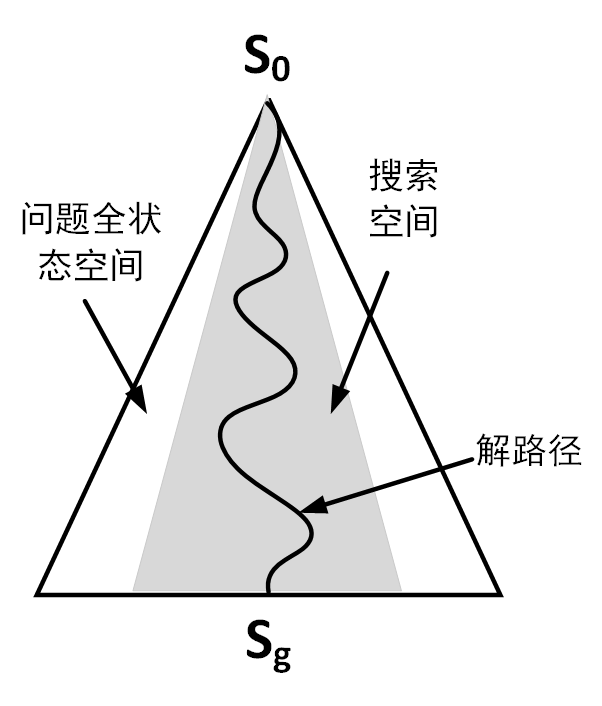
\includegraphics[width=0.3\textwidth,center]{fig/7-1.png}
\end{frame}
\begin{frame}{搜索算法分类}
    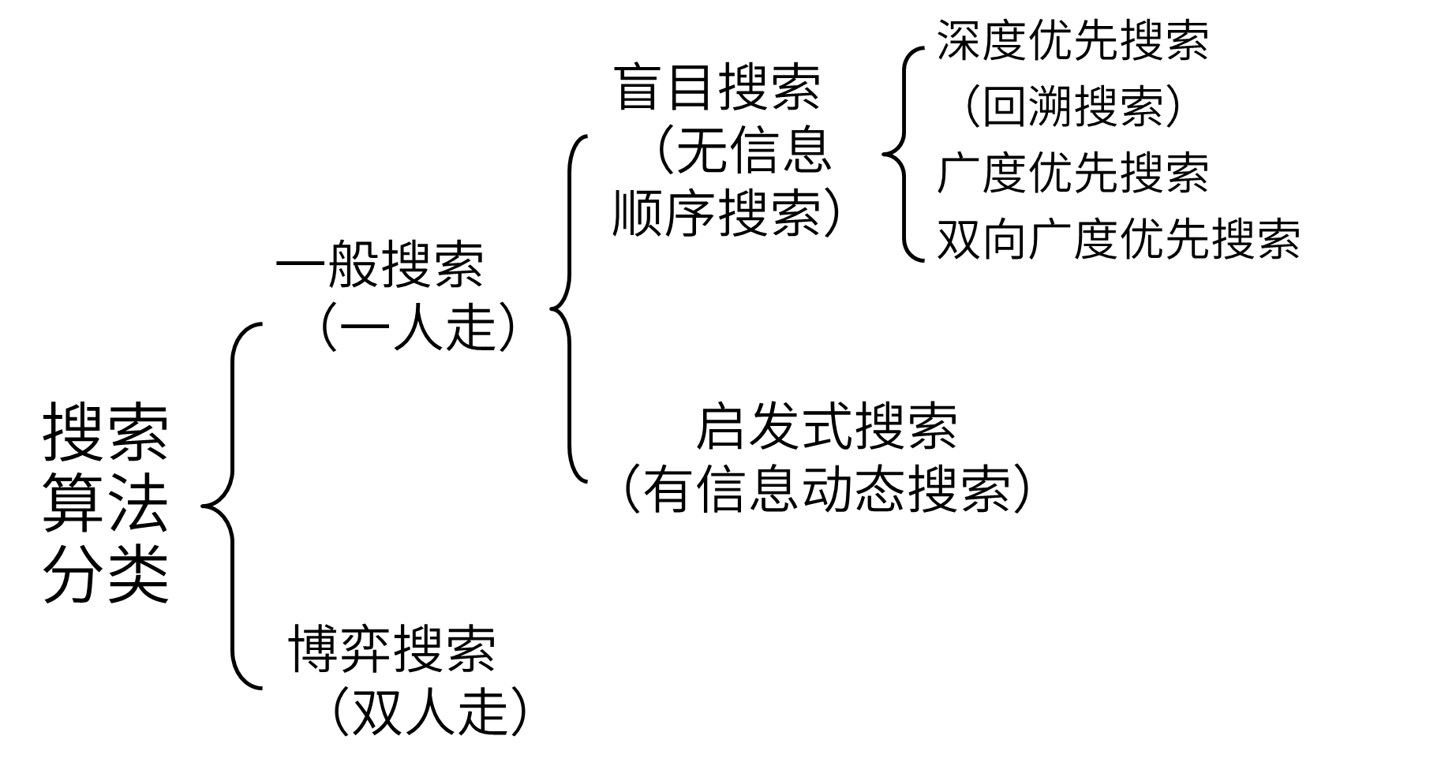
\includegraphics[width=0.9\textwidth,center]{fig/7-2.png}
\end{frame}
\begin{frame}{7.1 深度优先搜索}
    \begin{itemize}
        \item \textcolor{blue}{深度优先搜索}(Depth First Search, DFS)基本思想:从初始状态$S$开始,
        利用规则生成搜索树下一层任一个结点,检查是否出现目标状态$G$,若未出现,以此状态利用规则生成再下一层任一个结点,
        再检查是否为目标节点$G$,若未出现,继续以上操作过程,一直进行到叶节点(即不能再生成新状态节点),
        当它仍不是目标状态$G$时,\textcolor{blue}{回溯}(Backtracking) 到上一层结果,
        取另一可能扩展搜索的分支。生成新状态节点。若仍不是目标状态,就按该分支一直扩展到叶节点,若仍不是目标,
        采用相同的回溯办法回退到上层节点,扩展可能的分支生成新状态,……,一直进行下去,直到找到目标状态$G$为止
    \end{itemize}
\end{frame}
\begin{frame}{1011 -- Sticks (poj.org)}
    \begin{itemize}
        \item George took sticks of the same length and cut them randomly until all parts became at most 50 units long
        \item Now he wants to return sticks to the original state, but he forgot how many sticks he had originally and how long they were originally
        \item Please help him and design a program which computes the smallest possible original length of those sticks
        \item All lengths expressed in units are integers greater than zero
    \end{itemize}
    \begin{exampleblock}{例}
        \begin{itemize}
            \item 输入:5,2,1,5,2,1,5,2,1
            \item 输出:6
            \item 可能情况:24(5+5+5+2+2+2+1+1+1) 12(5+5+2,5+2+2+1+1+1) 8(5+2+1,5+2+1,5+2+1) 6(5+1,5+1,5+1,2+2+2)
        \end{itemize}
    \end{exampleblock}
\end{frame}    
\begin{frame}{7.2 广度优先搜索}
    \begin{itemize}
        \item \textcolor{blue}{广度优先搜索}(Breadth First Search, BFS) 基本思想:从初始状态$S$开始,利用规则生成所有可能的状态,构成树的下一层节点,检查是否出现目标状态$G$,若未出现,就对该层所有状态节点,分别顺序利用规则,生成再下一层的所有状态节点,对这一层的所有状态节点检查是否出现$G$,若未出现,继续按上面思想生成再下一层的所有状态节点,这样一层一层往下展开,直到出现目标状态为止
        \item 深度优先搜索(DFS)和广度优先搜索(BFS),不同的地方:
        \begin{itemize}
            \item DFS通常用来求可行解,判断路径是否存在;BFS通常来求最优路径
            \item DFS通常用递归(堆栈)来实现,而BFS通常用队列来实现
        \end{itemize}
    \end{itemize}
\end{frame}
\begin{frame}{1915 -- Knight Moves (poj.org)}
    \begin{itemize}
        \item \textcolor{blue}{骑士巡逻}(Knight‘s tour)问题
    \end{itemize}
    \vfill
    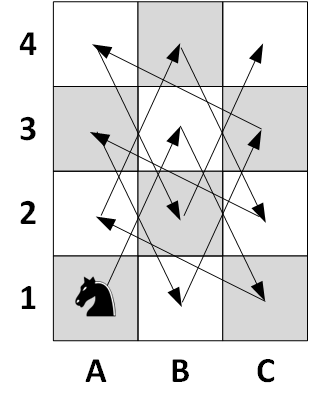
\includegraphics[width=0.3\textwidth,center]{fig/7-3.png}
\end{frame}
\begin{frame}{7.3 启发式搜索}
    \begin{itemize}
        \item 为了提高深度优先搜索或广度优先搜索的搜索效率,可以采用\textcolor{blue}{启发式搜索},使用\textcolor{blue}{最好优先贪心算法}和\textcolor{blue}{A*搜索算法}
        \item 最好优先算法定义一个评估$n$到目标节点的函数$h(n)$,在信息充足的情况下直接选择代价最低的节点
        \item A*算法则通过$g(n)+h(n)$来进行选择,$g(n)$是起点到$n$点的真实代价,而$h(n)$是$n$到终点的评估代价
        \item 设计合理的$h(n)$就可以提高算法效率并保证找到一条最优路径
    \end{itemize}
\end{frame}
\begin{frame}{1077 -- Eight (poj.org)}
    \begin{itemize}
        \item 经典的\textcolor{blue}{启发式搜索},使用\textcolor{blue}{数字推盘游戏}(n-puzzle) 游戏:从初始状态开始,到目标状态,每次有$2\sim4$种移动方式,每移动一次,又会产生新的状态,不管是深度优先搜索或者广度优先搜索,搜索的复杂性会逐渐增加,可以采用\textcolor{blue}{启发式搜索},使用\textcolor{blue}{最好优先贪心算法},通过设计合理的评估函数$h(n)$,每次计算函数值最优的值进行选择,进而提高算法效率
        \item 九宫格的状态构成了一个字符串序列,采用哈希算法的思想,将该字符串转化成一个数值,便于状态的保存
        \item \textcolor{blue}{启发式搜索},使用\textcolor{blue}{康托展开}能够将全排列和一个自然数进行映射,正好应用在该问题中,将$x$转换成9,这个字符串里面的字符正好对应1到9全排列中的一个
    \end{itemize}
\end{frame}
\begin{frame}{7.4 组合博弈}
    \begin{itemize}
        \item 一个典型的\textcolor{blue}{组合博弈}(Combinatorial game)问题,具有以下特征:
        \begin{enumerate}[(1)]
            \item 两个玩家(player)
            \item 游戏中有有限个可能的状态(position)
            \item 两个玩家遵从游戏规则,如果双方平等,称为无偏博弈(Impartial game)
            \item 两个玩家轮流行动
            \item 游戏到无法行动结束,通常情况下最后一个行动者获胜;如果是最后一个无法行动的玩家获胜,则称为Misère game;避免出现游戏结束不了造成的平局,会添加一个结束条件
            \item 游戏在有限次行动后结束
        \end{enumerate}
    \end{itemize}
\end{frame}
\begin{frame}{算法}
    \begin{itemize}
        \item 解决组合博弈问题,定义以下概念:
        \begin{itemize}
            \item 必败点(P-positions):使前一个玩家获胜的位置
            \item 必胜点(N-positions):使即将行动的玩家获胜的位置
            \item 结束点(terminal position):无法继续行动的位置
        \end{itemize}
        \item 有了以上定义,执行如下算法:
        \begin{enumerate}[(1)]
            \item 结束点为必败点
            \item 通过一次行动可以到达必败点的为必胜点
            \item 一次行动只能到达必胜点的为必败点
            \item 在(3)中无法找到新的必败点,就结束;否则转向(2)
        \end{enumerate}
    \end{itemize}
\end{frame}
\begin{frame}{2368 -- Buttons (poj.org)}
    \begin{itemize}
        \item 一个游戏有两个玩家,有一堆纽扣,数量是$k$,两个玩家轮流从纽扣堆中取走纽扣,每次取走至少1个,最多$n$个,取走最后一个纽扣者获胜
        \item 现在第二个取纽扣的玩家来决定$n$是多少,要求$2 \leq n < k$
        \item 问为了保证第二个玩家获胜,$n$的值最小是多少,如果找不到,$n$就为0
    \end{itemize}
    \begin{exampleblock}{例}
        3个纽扣,令$n=2$,则第一位玩家取1,第二位玩家取2;而第一位玩家取2,第二位玩家取1,第二位玩家都可以获胜
    \end{exampleblock}
\end{frame}
\begin{frame}{取子游戏}
    \begin{itemize}
        \item \textcolor{blue}{取子游戏}(subtraction game)
        \begin{enumerate}[(1)]
            \item 初始条件:1堆纽扣,数量为$k$
            \item 游戏规则:每次取走1到$n$个纽扣$(2\leq n < k)$
            \item 获胜条件:最后一个取走纽扣的玩家获胜
        \end{enumerate}
        \item $n=3$时,按照算法,0为结束点,是必败点(P);1,2,3可以分别通过取1,2,3个纽扣到达0的位置,所以它们是必胜点(N)
        \item $n=4$时,无论取几个纽扣,到达的都是N点,所以4为必败点,依此类推,如图所示
        \vfill
        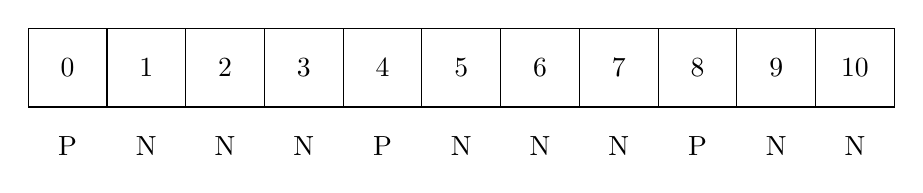
\begin{tikzpicture}
            \foreach \x in {0,1,...,10}
                \node[RA2] at (\x,0) {\x};
            \foreach \y[count=\i] in {P,N,N,N,P,N,N,N,P,N,N}
                \node at (\i-1,-1) {\y};    
        \end{tikzpicture}
        \item 不难发现,凡是$n+1$整数倍的位置都是P点,其他位置是N点,第二位玩家获胜,只需将$n$设置为$k\%(n+1)=0$即可   
    \end{itemize}
\end{frame}
\begin{frame}{2975 -- Nim (poj.org)}
    \begin{itemize}
        \item \textcolor{blue}{Nim游戏}
        \begin{enumerate}[(1)]
            \item 初始条件:$n$堆石子,第$i$堆石子的数量为$k[i]$
            \item 游戏规则:选择任意一堆,从该堆取走1个以上石子
            \item 获胜条件:所有石子被取走,最后一个取石子的玩家获胜
        \end{enumerate}
        \item 每堆的剩余数量$k[i]$用二进制表示,当且仅当所有的$k[i]$进行异或运算的结果为0时是必败点,即$k[1]\oplus k[2]\oplus \ldots \oplus k[n]=0$
        \item 例如3堆石子,数量为$7,11,13$,转化为二进制进行异或运算:$(111)_2\oplus (1011)_2\oplus (1101)_2=(1)_2$,所以此位置是必胜点
        \item 本题求Nim游戏中,给定初始状态下,能够获胜的取子方法有几种   
    \end{itemize}
\end{frame}
\end{document}